\documentclass{report}
\usepackage[a4paper, margin=0.5in]{geometry}
\usepackage{parskip}
\usepackage{graphicx}
\usepackage{caption}
\usepackage{amssymb}
\usepackage{amsmath}
\usepackage{algpseudocode}
\usepackage{algorithm}

\captionsetup[figure]{
  font = it,
  labelfont = bf
}

\begin{document}
  \begin{minipage}[b]{0.48\textwidth}
    \section*{Load balancing in standard kMeans}
    Suppose that the standard kMeans algorithm is executed in parallel by splitting between T threads the total points N. In this case the work load is easly divided equally between the threads. In fact we can calculate the total number of points to assign each thread by N/T; if N is not a multiple of T we will also have a reminder
    \begin{equation}
      reminder = N \text{ mod } T < T
    \end{equation}
    If this is the case, we can simply assign the first threads one more point, therefore in the end there will be r threads with N/T + 1 points and T - reminder threads with N/T points.

    \section*{Load balancing in Hamerly's algorithm}
    With Hamerly's algorithm, efficient load balancing is not as easy as in the standard version because, for every cycle, it is not neccessary to compute the distances for every points but only for critical ones. Because of this, if the points were simply divided among the threads, it might happen that some have many points while others could have few calculations to do.

    \begin{center}
      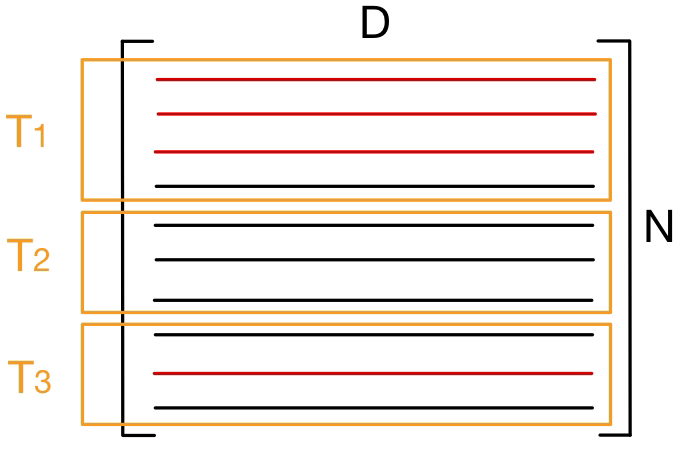
\includegraphics[width = 0.8\textwidth]{imgs/non_balances_hamerly.png}
      \captionof{figure}{Non balanced point division}
      \label{fig:non_bal_ham}
    \end{center}

    The Figure \ref{fig:non_bal_ham} shows an input matrix (N x d, where d is the data dimensionality) where critical points are not  equally distribuited. In this case, the first thread will have three critical points whereas the second thread will have zero.

    To implement an efficient load balacing, a more advanced strategy is needed and one possible solution will be presented in the following part of this report. 
    
    \subsection*{Points assigment for Hamerly's algorithm}
    First of all remember that, in the Hamerly's algorithm, after that each centroid moved it is neccessary to update the upper bound (ub) and the lower bound ($lb$) of each p. This operation can be done in parallel, since the update is indipendent between the points, and the work that has to be done is equal for each p. 

    During this phase, each thread will have a linked list where they add every critical point that it finds, moreover every time it finds a critical it increments by one the value of a global array which has a length of T so that each thread has its own index to access.

    After that all points have been iterated a synchronization is required. During this sequential part it is calculated the total number of critical points (C) that have been found and a second array is created with a length of C.
  \end{minipage}
  \hspace{0.15in}
  \raisebox{0in}{
  \begin{minipage}[b]{0.48\textwidth}
    At this point, every thread can insert, inside this new array, its critical points. In order to do that, every thread has to start inserting its values from the index which is equal to the sum of the number of criticals found by the previous threads.

    For example, if there are 3 threads and they found respectively [2, 3, 1] criticals then, they start inserting values from the 0, 2 and 5 (2 + 3) index. The objective of this step is to create an array containing all the critical points together because in this way it is possible to equally divide those critical between the threads. 

    If the total number of critical points is $C$ then, the number of criticals to assign each thread can be calculated as $C / T$. If $C$ is not a multiple of T, there will also be a remainder which can be handled the same way as in the standard case. Below is the pseudo code where N is the total numer of points and "points" is the array containing all points.

    \begin{algorithm}[H]
      \caption{Boundaries update pseudo-code}\label{alg:cap}
      \begin{algorithmic}
        \State --------------------------------------------- \Comment Sequentially
        \State Let nC be the array with the number of criticals found by each thread 
        \State remainder = N \% T
        \State --------------------------------------------- \Comment In Parallel
        \State Let criticals\_per\_thread be the local list of criticals found by the thread

        \State$p\_per\_thread = Int(N/T)$
        \State offset = remainder

        \If{$thread\_id < remainder$}
          \State $p\_per\_thread = p\_per\_thread + 1$
          \State offset = 0
        \EndIf

        \State
        \For{$j < p\_per\_thread$}
          \State p = points[p\_per\_thread $\cdot$ thread\_id + offset + j]
          \State p.ub = p.ub + cdistaces[p.centroid\_index]
          \If{p.centroid\_index == maxdist\_index}
            \State p.lb = p.lb - secmaxdist
          \Else
            \State p.lb = p.lb - maxdist
          \EndIf

          \If{p.$ub>$ p.lb}
            \State criticals\_in\_thread.push(p)
            \State nC[thread\_id] = nC[thread\_id] + 1
          \EndIf
        \EndFor
        \State --------------------------------------------- \Comment Sequentially 
        \State C = 0
        \For{j $<$ nC.length}
          \State C = C + nC[j]
        \EndFor

        \State Let criticals be the array of all the criticals
        \State --------------------------------------------- \Comment In Parallel 
        \State index = 0
        \For{j $<$ i}
          \State index = index + nC[j]
        \EndFor
        \State 
        \For{j $<$ nC[i]}
          \State criticals[index + j] = criticals\_per\_thread.pop 
        \EndFor
      \end{algorithmic}
  \end{algorithm}
  \end{minipage}}

  \newpage

  \begin{minipage}[b]{0.48\textwidth}
    \subsection*{Insight into the opseudo code}
    Because some of the steps in the pseudocode may not be immediate in understanding what they do and why they are used, this part will give an overview of those instructions that may be less clear.
    \begin{algorithm}[H]
      \caption{$N_i$ increment}
      \begin{algorithmic}
        \If{$thread\_id < remainder$}
          \State $p\_per\_thread = p\_per\_thread + 1$
        \EndIf
      \end{algorithmic}
    \end{algorithm}

    This if statement is implemented to increase by one the number of points that the first threads have to access.

    \begin{algorithm}[H]
      \caption{p.centroid.distance}
      \begin{algorithmic}
        \State p.ub = p.ub + cdistances[p.centroid\_index]
      \end{algorithmic}
    \end{algorithm}

    Through cdistances[p.centroid\_index] we access distance traveled by the centroid to which the point has been assigned.

    At every iteration the upper bound of each point, which is accessed by p.ub, has to be updated and the new value will be: p.ub + cdistances[p.centroid\_index]

    \begin{algorithm}[H]
      \caption{lower bound update}
      \begin{algorithmic}
        \If{p.centroid\_index == maxdist\_index}
          \State p.lb = p.lb - secmaxdist
        \Else
          \State p.lb = p.lb - maxdist
        \EndIf
      \end{algorithmic}
    \end{algorithm}

    When it comes to updating the lower limit, the first thing to check is whether the centroid that moved the most is also the one assigned to the p. In this case, the lower limit cannot be updated with the distance of that centroid because it has already been used for the upper limit, but in this case the distance taken from the second centroid that moved the most has to be used.

    \begin{algorithm}[H]
      \caption{lower bound update}
      \begin{algorithmic}
        \State index = 0
        \For{j $<$ thread\_id}
          \State index = index + nC[j]
        \EndFor
      \end{algorithmic}
    \end{algorithm}

    This is the part where each thread calculate the index from where it has to start inserting the vales in the global array containing all the critical points.

    \begin{algorithm}[H]
      \caption{add values to the global array}
      \begin{algorithmic}
        \For{j $<$ nC[i]}
          \State criticals[index + j] = $L_i$.pop 
        \EndFor       
      \end{algorithmic}
    \end{algorithm}
    This is the last part of the algorithm where every thread inserts into the global array the value of its list.
  \end{minipage}
  \hspace{0.1in}
  \raisebox{2.5in}{
  \begin{minipage}[b]{0.48\textwidth}
  \end{minipage}}
\end{document}